\section{Faithfulness Beyond Reconstruction}\label{sec:beyond}

The base SAEs reconstruct GPT-2 activations with 76--95\,\% explained variance. This section asks what that
reconstruction preserves at the other three levels. All results in this section are \evlabel{validation} findings
unless marked otherwise.

\subsection{Information faithfulness}\label{sec:info}

\paragraph{Frozen readers overstate the loss of truth information.} A logistic truth probe fitted on original
activations and applied unchanged to SAE reconstructions loses 0.28--0.29 AUROC on GoT (Table~\ref{tab:m2},
Figure~\ref{fig:m2}). Taken at face value, this would suggest that the reconstructions discard most of the truth
signal. The norm-matched noise reference shows otherwise: adding isotropic noise with the same norm as the SAE error
produces almost the same drop (0.25--0.26), and a simpler mass-mean reader loses only 0.02--0.03. Most of the
frozen-probe collapse therefore reflects the sensitivity of that particular reader to any perturbation of this size,
not information that the SAE specifically removed.

\paragraph{A smaller loss of truth information remains.} Readers re-trained on the reconstructions are 0.07--0.12
AUROC worse than readers trained on original activations. Re-training never recovers the original performance, so no
cell is classified as preserved, and the task label can be decoded from the reconstruction error alone (AUROC
0.62--0.68 on GoT). Some truth information is thus still present in the activation but outside the SAE's
reconstruction. Re-trained readers provide the stricter and more relevant test of whether information is retained,
and the frozen reader is better understood as a test of whether an existing readout still works.

\paragraph{Persona information is lost, not only misread.} The persona task behaves differently. On the
equal-length RepE-LM prompts, the frozen persona gap (0.10--0.24) is 1.9--3.4 times the gap caused by norm-matched
noise, and re-trained readers recover little of it: the re-trained gap is 0.08--0.22, and its statement-bootstrap
interval excludes zero for all 99 base SAEs at layers 1--11 (Appendix Table~\ref{tab:rlm_layers}). Part of this loss
is generic, because a neutral one-word swap also loses information, but at layers 2--8 the persona gap exceeds the
neutral control by 0.06--0.12, so part of the mid-layer loss is persona-specific. The geometry of the persona contrast
is also distorted. For each pair, the reconstructed honest-minus-dishonest difference
$\hat\Delta=\hat{x}_H-\hat{x}_U$ has a cosine of only 0.35--0.58 with the original difference $\Delta=x_H-x_U$, although
the mean difference direction over all pairs is kept better (cosine 0.70--0.86). The SAE reconstructs each prompt of
a pair reasonably well while reconstructing their difference poorly, because the two reconstruction errors do not
cancel.

\paragraph{The PCA verdict depends on how PCA is constrained.} A natural question is whether an SAE preserves task
information better than a dense linear reconstruction. When PCA is matched to the SAE's OWT reconstruction error, PCA
keeps at least as much information in every cell, and the SAE is significantly worse in 52 of 81 GoT cells, 59 of 99
persona cells and 81 of 90 neutral cells. In the pre-registered PCA-CM replication on the 20 trained family$\times$layer
cells, the SAE is worse in 13 and never better (Table~\ref{tab:pcacm}). That comparison, however, gives PCA 298--519
dense components, whereas every SAE activates about 128 latents per token. When PCA is restricted to the same
per-token budget ($k=128$), no trained SAE is classified worse and three of 20 cells are better; when $k$ is matched to
each SAE's mean task-level activity ($k=54$--128), eight are better and none worse. Under an approximate post-hoc Holm
correction over the 40 capacity-matched cells, one of the three $k=128$ cells and four of the eight task-matched cells
remain. ``Not worse'' does not mean equivalent: the pre-registered $\pm0.02$ equivalence class is met in none of the
40 cells, because the paired intervals are wider than the margin. Whether an SAE preserves more or less information
than PCA is therefore not a property of the SAE alone; it depends on whether the comparison equalises reconstruction
error or the number of active dimensions. The persona and neutral tasks have been compared at equal error only.

\paragraph{Architecture differences are confounded.} On truth, ReLU loses least and JumpReLU most under re-trained
readers, the reverse of the reconstruction ranking; on persona, ReLU loses most. Because task-level L0 is not matched
across architectures (Section~\ref{sec:recon}), and an exploratory control that truncates each token to its 128
largest latents moves JumpReLU's persona gap substantially while leaving ReLU nearly unchanged, we do not rank
architectures on information preservation.

% generated by scripts/shared/build_paper_artifacts.py from results/shared/m2_four_level_faithfulness/summary_by_layer_arch.csv
\begin{table}[t]
\centering
\small
\caption{M2 information preservation (VALIDATION): AUROC gaps (original $-$ reconstructed; $\downarrow$), mean over informative layers (GoT 4--11, RepE-LM 1--11) and 3 seeds. ``Noise'' adds isotropic noise with the norm of the SAE error; ``PCA'' is matched to the SAE's OWT validation NMSE. Error AUROC: label decoded from the error term alone. Source: \texttt{results/\allowbreak{}shared/\allowbreak{}m2\_four\_level\_faithfulness/\allowbreak{}summary\_by\_layer\_arch.csv}.}
\label{tab:m2}
\begin{adjustbox}{max width=\linewidth}
\begin{tabular}{llccccccc}
\toprule
Task & SAE & Frozen log. & Noise & Frozen m.-mean & Re-trained log. & PCA re-tr. & MLP & Error AUROC \\
\midrule
GoT & ReLU & 0.287 & 0.259 & 0.033 & 0.066 & 0.042 & 0.049 & 0.675 \\
GoT & TopK & 0.275 & 0.246 & 0.024 & 0.075 & 0.032 & 0.037 & 0.615 \\
GoT & JumpReLU & 0.286 & 0.257 & 0.026 & 0.118 & 0.030 & 0.066 & 0.632 \\
\midrule
Persona & ReLU & 0.198 & 0.076 & 0.091 & 0.179 & 0.131 & 0.232 & 0.773 \\
Persona & TopK & 0.162 & 0.072 & 0.066 & 0.147 & 0.116 & 0.190 & 0.719 \\
Persona & JumpReLU & 0.155 & 0.064 & 0.062 & 0.143 & 0.114 & 0.177 & 0.721 \\
\midrule
Neutral & ReLU & 0.113 & 0.048 & 0.049 & 0.099 & 0.066 & 0.033 & 0.636 \\
Neutral & TopK & 0.098 & 0.046 & 0.038 & 0.090 & 0.064 & 0.031 & 0.615 \\
Neutral & JumpReLU & 0.094 & 0.043 & 0.035 & 0.083 & 0.062 & 0.031 & 0.619 \\
\bottomrule
\end{tabular}
\end{adjustbox}
\end{table}


\begin{figure}[t]
  \centering
  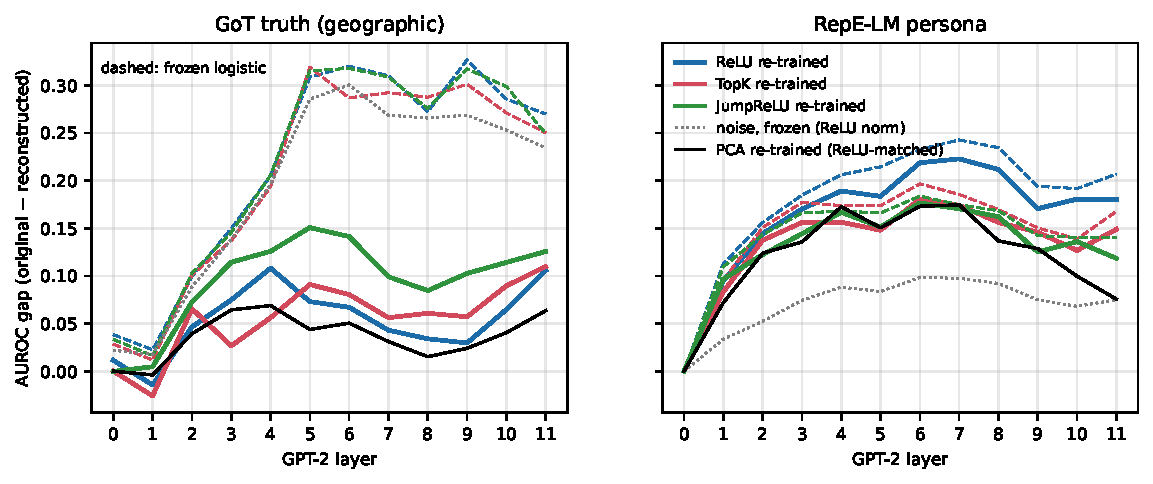
\includegraphics[width=\linewidth]{fig_m2_information}
  \caption{Information preservation by layer for the base GPT-2 SAEs (\evlabel{validation}). Dashed lines: frozen
  logistic AUROC gap; solid lines: re-trained logistic gap; dotted grey: frozen gap under norm-matched noise; black: PCA
  matched to the ReLU SAE's reconstruction error.}
  \label{fig:m2}
\end{figure}

% generated by scripts/shared/pca_cm_posthoc_multiplicity.py from results/shared/pca_capacity_matched/
\begin{table}[t]
\centering
\small
\caption{PCA-CM (\evlabel{validation}; GoT cities+neg\_cities VAL, 448 rows): SAE vs PCA on the GoT re-fit logistic truth gap (lower is better) under three matching constraints, over the 20 trained family$\times$layer cells (L8, L11; random decoder excluded). ``Better''/``worse'': every seed's paired 95\,\% grouped-bootstrap CI excludes zero (pre-registered rule, no correction across cells). ``Holm'': cells that also survive an approximate post-hoc Holm correction over the 40 capacity-matched cells. Better at $k=128$ (SAE vs PCA gap): L8 R2 ReLU: 0.012 vs 0.058; L8 res-jb: 0.025 vs 0.058; L11 R2 ReLU: 0.076 vs 0.153.}
\label{tab:pcacm}
\begin{adjustbox}{max width=\linewidth}
\begin{tabular}{lccccc}
\toprule
PCA reference & PCA $k$ & SAE better & of which Holm & inconclusive & SAE worse \\
\midrule
Equal OWT error (existing reference) & 298--519 & 0 & -- & 7 & 13 \\
Fixed $k=128$ (per-token active budget) & 128 & 3 & 1 & 17 & 0 \\
$k$ = SAE's GoT task L0 & 54--128 & 8 & 4 & 12 & 0 \\
\bottomrule
\end{tabular}
\end{adjustbox}
\end{table}


\subsection{Behavioural faithfulness}\label{sec:behaviour}

\paragraph{Splicing damage grows with depth.} Splicing the reconstruction into GPT-2 at every non-BOS position
increases next-token cross-entropy by 0.009--0.026 nats at layer 1 and by 0.213--0.358 nats at layer 11
(Appendix Table~\ref{tab:splice}; Figure~\ref{fig:recon}, right). Loss recovered relative to mean ablation stays at or
above 0.93, and an identity splice changes nothing, which validates the hook. The model's preference for true over
false GoT statements (0.82 originally) is unchanged within $\pm0.025$ through layer 8 and drops by 0.04--0.09 at
layers 9--11.

\paragraph{SAE error is usually more harmful than random error of the same size.} Replacing the SAE error by a
norm-matched random error gives a smaller cross-entropy increase in most runs. The ratio of SAE-induced to
random-induced damage is 0.76--2.89 per run (median 1.64), and the seven runs below 1 are all at layers 1--3. We read
this ratio cautiously: it shows that the SAE error is not behaviourally neutral and is concentrated in directions the
downstream computation is sensitive to, but it does not identify which directions those are or why.

\paragraph{Within a layer, reconstruction error predicts behavioural damage but not truth loss.} Pooling SAEs across
layers mixes the depth trend with differences between SAEs and inflates correlations. The M0 reanalysis therefore
regresses each outcome on reconstruction error within layer, with layer and architecture fixed effects and a
within-layer permutation test (Table~\ref{tab:m0}). Lower OWT NMSE predicts less splice damage
($\beta=0.165$ per unit log NMSE, Holm-corrected $p=0.0008$; per-layer Spearman $\rho$ 0.80--0.97 from layer 3), and the
association survives without architecture fixed effects. For the frozen GoT truth gap, the formal test passes (Holm
$p=0.044$), but architecture explains 99.8\,\% of the within-layer NMSE variance and the association disappears
without architecture fixed effects ($p=0.89$). Reconstruction error measured on the GoT statements themselves is
not supported as a predictor of either outcome in the primary model (Holm $p=1.0$ for both). Reconstruction error is therefore a robust within-layer predictor of behavioural
damage and not a robust predictor of truth-information loss. The same analysis corrects an earlier claim: a pooled
correlation of 0.89 between reconstruction quality and persona preservation falls to 0.05 within layer.

% generated by scripts/shared/build_paper_artifacts.py from results/shared/m0_within_layer_reanalysis/within_layer_regressions.csv
\begin{table}[t]
\centering
\small
\caption{M0 within-layer regressions (VALIDATION): outcome $\sim\beta\cdot$predictor + layer FE + architecture FE + log L0, Freedman--Lane permutation within layer. The GoT row passes formally but vanishes without architecture fixed effects ($p=0.89$; see text). Source: \texttt{results/\allowbreak{}shared/\allowbreak{}m0\_within\_layer\_reanalysis/\allowbreak{}within\_layer\_regressions.csv}.}
\label{tab:m0}
\begin{adjustbox}{max width=\linewidth}
\begin{tabular}{lccccc}
\toprule
Predictor $\rightarrow$ outcome & $\beta$ & 95\% CI & $p_{\text{perm}}$ & $p_{\text{Holm}}$ & $n$ \\
\midrule
log OWT NMSE $\rightarrow$ GoT frozen-logistic gap & 0.268 & [0.056, 0.477] & 0.0146 & 0.0438 & 72 \\
log GoT relative error $\rightarrow$ GoT frozen-logistic gap & 0.005 & [-0.059, 0.080] & 0.8680 & 1.0000 & 72 \\
log OWT NMSE $\rightarrow$ OWT spliced $\Delta$CE & 0.165 & [0.134, 0.265] & 0.0002 & 0.0008 & 107 \\
log GoT relative error $\rightarrow$ OWT spliced $\Delta$CE & -0.012 & [-0.060, 0.028] & 0.6267 & 1.0000 & 107 \\
\bottomrule
\end{tabular}
\end{adjustbox}
\end{table}


\subsection{Causal site and causal preservation}\label{sec:causal}

\paragraph{Where GPT-2 carries the persona effect (M3).} Before asking whether the SAE preserves a causal effect, we
locate one in the original model. For each RepE-LM pair, the honest and dishonest prompts change the next-token
distribution by a mean $\mathrm{KL}(p_H\|p_U)$ of 0.033 nats. Copying the honest activation into the dishonest run at
one layer and position group restores a share of that divergence. The effect is carried by the persona word early
(share 0.97 at the layer-1 persona slot) and by the final token late (0.95 at layer 11), with the handover at layers
7--8 (Figure~\ref{fig:m3}). Of 65 cells, 50 pass the pre-registered test against 200 matched-norm random vectors with
Holm correction. The sites were selected on training prompts and replicated on validation prompts: the layer-1 persona
slot and the layer-11 final token by the pre-registered rule, and the layer-8 final token by a pre-registered
amendment. A same-meaning synonym swap travels the same route at about half the size, and template T1 has no effect
beyond its synonym control, so T2--T4 form the primary set.

\paragraph{How much of the effect the reconstruction retains (M4).} At a site, the activation difference splits
exactly into a reconstructed part and an error part, $\Delta=\Delta_{\text{rec}}+\Delta_{\text{err}}$. With
$T(v)=\mathrm{KL}(p_H\|p_U)-\mathrm{KL}(p_H\|p_{U+v})$ we compare $T_{\text{full}}=T(\Delta)$ with
$T_{\text{rec}}=T(\Delta_{\text{rec}})$, $T_{\text{err}}=T(\Delta_{\text{err}})$ and the interaction
$I=T_{\text{full}}-T_{\text{rec}}-T_{\text{err}}$. The reconstructed difference restores 93--97\,\% of the effect at the
layer-1 persona slot but only 62--68\,\% at the layer-8 and layer-11 final token (Table~\ref{tab:m4},
Figure~\ref{fig:m4}). At those later sites, ReLU's error part alone carries 40--45\,\%, and for TopK and JumpReLU the
interaction is large ($|I|/T_{\text{full}}$ 0.26--0.38), so their shares cannot be read additively. Higher explained
variance does not imply higher causal preservation: at layer 11, TopK has higher EV than ReLU (0.815 versus 0.757) but
retains less of the effect (0.62 versus 0.68).

\paragraph{What the patching design does and does not show.} Patching the top-$k$ SAE latents (setting the dishonest
prompt's selected latents to their honest values and keeping the error term) restores more of the effect than 200
frequency- and magnitude-matched random latent sets for every SAE and site ($p=0.005$, the minimum attainable). The
effect is distributed: one latent carries 2--10\,\% of $T_{\text{rec}}$ and 64 latents carry 47--74\,\%. Because the
error term is kept, however, every such patch is equivalent to adding a single vector $v=W_d(z'-z_U)$ to the dishonest
prompt's original activation, and a dictionary of 3{,}072 latents spans the residual stream, so lying in decoder space
does not restrict $v$. What is SAE-specific is how $v$ is chosen: the encoder's input-dependent selection of latents.
The design therefore shows that the SAE \emph{selects} directions that carry the effect when inserted and measures how
much of the effect the reconstruction \emph{preserves} under this intervention structure. It is not a mediation
analysis: it does not show that the model's downstream computation passes through SAE latents, which would require
the computation to run through SAE nonlinearities, for example with SAEs spliced at later layers or without the error
term. A layer-6 clamp experiment of that kind found no supported effect (\evlabel{validation}), and a pre-registered
mediated SAE-in-the-loop experiment has not been run.

\paragraph{A low-rank reference.} To give the M4 shares a reference point, R5 compares SAE patches with supervised and
unsupervised subspaces of matched rank at the same sites (\evlabel{validation}, descriptive; Appendix
Table~\ref{tab:r5}). The persona effect is low-rank: one learned direction carries 0.92 of it at layer 1, 0.64 at
layer 8 and 0.40 at layer 11, and four learned directions carry 1.02, 0.91 and 0.62. At layer 8 a rank-4 learned
subspace carries more of the effect than the whole SAE reconstruction (0.91 versus 0.62--0.67), whereas random
subspaces carry at most 0.13 even at rank 64. The partial preservation at later sites is therefore a property of the
SAE basis, not of the task; the SAE basis is far from the best basis of matched rank, although it is well above random.

\paragraph{Sensitivity.} The persona effect is small ($T_{\text{full}}=0.022$ nats at the layer-8 final token), so one
SAE's preservation share can only be resolved to 0.054--0.107 there (0.013--0.017 at layer 1 and 0.036--0.069 at layer
11). Differences between SAEs smaller than this at layer 8 are not interpretable.

\begin{figure}[t]
  \centering
  \begin{minipage}[t]{0.49\linewidth}
    \centering
    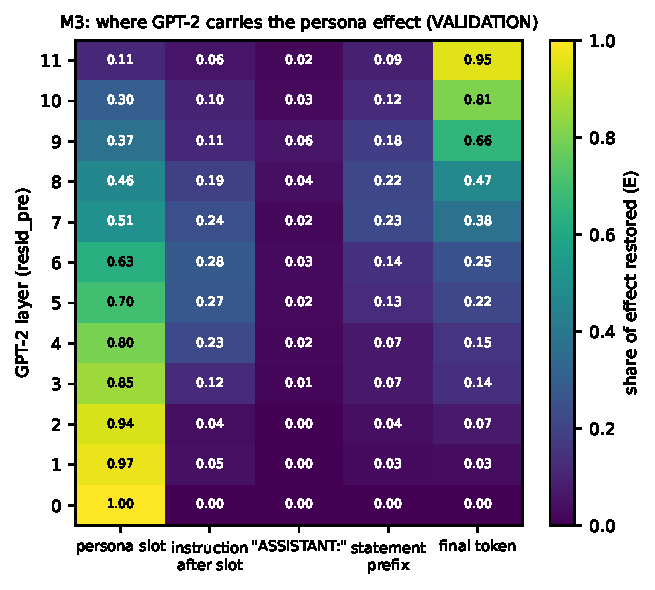
\includegraphics[width=\linewidth]{fig_m3_sites}
  \end{minipage}\hfill
  \begin{minipage}[t]{0.49\linewidth}
    \centering
    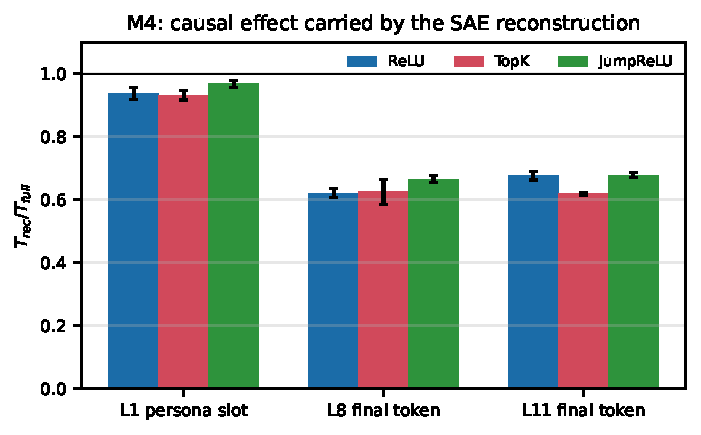
\includegraphics[width=\linewidth]{fig_m4_preservation}
  \end{minipage}
  \caption{Causal site and causal preservation in GPT-2 Small (\evlabel{validation}). Left (M3): share of the
  persona-instruction effect restored by patching one position group at one layer of the original model. Right (M4):
  share of the effect carried by the SAE-reconstructed activation difference, $T_{\text{rec}}/T_{\text{full}}$, at the
  three selected sites (mean $\pm$ sd over 3 seeds; templates T2--T4).}
  \label{fig:m3}\label{fig:m4}
\end{figure}

% generated by scripts/shared/build_paper_artifacts.py from results/repe/sae_patch_decomposition/architecture_summary.csv
\begin{table}[t]
\centering
\small
\caption{M4 causal decomposition (VALIDATION; templates T2--T4; mean$\pm$sd over 3 seeds). Shapley shares in parentheses are not interpretable as additive (pre-registered rule: interaction too large). Source: \texttt{results/repe/sae\_patch\_decomposition/architecture\_summary.csv}.}
\label{tab:m4}
\begin{adjustbox}{max width=\linewidth}
\begin{tabular}{llccccc}
\toprule
Site & SAE & $T_{\text{full}}$ (nats) & $T_{\text{rec}}/T_{\text{full}}$ & $T_{\text{err}}/T_{\text{full}}$ & $|I|/T_{\text{full}}$ & $\phi_{\text{rec}}$ \\
\midrule
L1 persona slot & ReLU & 0.0435 & 0.938$\pm$0.019 & 0.14 & 0.12 & 0.90 \\
 & TopK & 0.0435 & 0.931$\pm$0.014 & 0.16 & 0.14 & 0.89 \\
 & JumpReLU & 0.0435 & 0.968$\pm$0.011 & 0.03 & 0.10 & 0.97 \\
L8 final token & ReLU & 0.0220 & 0.621$\pm$0.015 & 0.45 & 0.12 & 0.59 \\
 & TopK & 0.0220 & 0.625$\pm$0.039 & 0.09 & 0.32 & (0.77) \\
 & JumpReLU & 0.0220 & 0.665$\pm$0.011 & 0.11 & 0.26 & (0.78) \\
L11 final token & ReLU & 0.0430 & 0.677$\pm$0.014 & 0.40 & 0.16 & 0.64 \\
 & TopK & 0.0430 & 0.620$\pm$0.004 & 0.06 & 0.38 & (0.78) \\
 & JumpReLU & 0.0430 & 0.678$\pm$0.007 & 0.11 & 0.28 & (0.78) \\
\bottomrule
\end{tabular}
\end{adjustbox}
\end{table}


\subsection{Relationship between the four levels}\label{sec:relationship}

Taken together, the GPT-2 evidence shows that the four levels move together in some respects and apart in others.
Reconstruction and behaviour are closely linked: within a layer, an SAE with lower reconstruction error damages
next-token prediction less, and the splice damage grows with depth as reconstruction degrades. Reconstruction and
information are only loosely linked: truth-information loss is not robustly predicted by reconstruction error within a
layer, the apparent truth collapse under frozen readers is mostly reader fragility, and persona information is lost
even by SAEs that reconstruct well. Reconstruction and causal preservation can disagree directly, as the layer-11
comparison of TopK and ReLU shows, and at later sites about a third of a causal effect that the model demonstrably uses
lies outside the reconstructed difference. A single reconstruction number cannot summarise these patterns, because
the levels respond to different parts of the activation: reconstruction to the high-variance bulk, behaviour to
whatever downstream computation reads, information and causal preservation to small, task-specific differences
between nearly identical activations.
